\chapter{General Discussion}
\section{Toward a molecular characterization of ocular dominance}
In chapter 2, I presented a a novel tissue sampling strategy for the elucidation of molecular correlates of visual development.  This strategy centers around the study of ocular dominance in the developing ferret.  Through a combination of dissection, fluorescent tracer, and in vivo imaging experiments, I show that it is possible to isolate structures in the retina, LGN, and cortex that form the anatomical basis of ocular dominance.  These samples were then used as the substrate for proteomic analysis using two dimensional difference gel electrophoresis (2D-DIGE) and matrix assisted LASER desorbtion/ionization time of flight (MALDI-TOF) mass spectroscopy.  We identified molecular candidates from the retina, LGN, and visual cortex that may contribute to the formation and/or maintenance of ocular dominance columns in the ferret.  

The tissue sampling strategy employed in chapter 2 could be easily used as the sample generation scheme for other screens targeted at providing a genetic characterization of ocular dominance.  In the past, differential mRNA display (Corriveau et al., 1998), DNA microarrays (Tropea et al., 2006), and 2D-DIGE (Van den Bergh et al., 2006a) have been successfully employed in the study of visual development.  All of these screens share a basic common methodology in that they are comparisons of two sample pools to one another.  I show that it is possible to generate pairs of samples in the retina, LGN, and cortex such that ocular dominance may be explored.  These samples could be processed with the above techniques to yield further insights into the establishment and/of maintenance of ocular dominance at the level of mRNA expression or at the level of protein expression. 

The choice of an appropriate screen for use with the tissue sampling strategy presented in this dissertation will depend on the experimental goals at hand.  The use of a gel based screening system such as the 2D-DIGE system presented here leads to one fundamental advantage over many other screens.  Gel based methods operate at the protein level where many other methods operate at the mRNA level.  As a result, gel based techniques are capable of directly measuring differences in protein expression across samples where other techniques force the experimenter to infer protein expression levels from mRNA levels.  Due to the direct measurement of protein expression, a more fine grained analysis of the samples is permitted.  Specifically, differential regulation of mRNA expression or splice variants across samples will be shown in a proteomic screen but not in other techniques based on mRNA.  Additionally, studies such as those using DNA microarrays followed by RT-PCR frequently suffer from a high signal to noise ratios and can be difficult to interpret because of this (Murray et al., 2008). Gel based techniques such as the one presented here do not rely on amplification methods and typically show a much better signal to noise ratio with detection limits as low as 0.5 fmol of protein (Unlu et al., 1997; Gong et al., 2004; Viswanathan et al., 2006). However, gel based methods provide less coverage across the genome of samples than other techniques based on an unbiased screens of mRNA.  Making use of the 2D-DIGE system presented here, membrane bound proteins are underrepresented in my resultant data due to a bias of 2D-DIGE toward cytosolic proteins during the IEF separation phase of the experiment.  Other two dimensional gel techniques involving doubled SDS-PAGE separation rather than the IEF/SDS-PAGE approach taken here have been developed in order to include membrane bound proteins (Rais et al., 2004), but  these methods suffer from poor mass resolution when compared to standard IEF/SDS-PAGE techniques. As a result doubled SDS-PAGE methods are not particularly useful for comparative screens in which only small proteomic changes are expected.  

For the molecular characterization of ocular dominance using the tissue strategy provided here, 2D-DIGE appears to be a good choice of screening system.  The proteomic changes across retina, LGN, and visual cortex sample pairs can be rather small and as such it is important to choose a system that is capable of detecting subtle expression differences.  These changes may not be apparent in other techniques where signal to noise is higher.  Changes may also manifest themselves at the level of protein expression and slice variation.  Again, the ability of 2D-DIGE to detect these changes makes it a good choice of screening system.  2D-DIGE does suffer from bias away from membrane bound proteins and the data recovered from these experiments must be interpreted in this light. 

Beyond the choice of methodology selected, the choice of animal model will impact both the scope and quality of experiments implementing the tissue sampling strategy presented here.  The majority of the work that was carried out in this dissertation was done in the ferret,  but these methods are directly translatable to many other mammalian models.  In the case of the retina and the LGN, it is possible to generate samples for comparison of ocular dominance at the molecular level in any rodent, carnivore, or primate.  The anatomy of the retina and LGN that allows us to isolate these samples in the ferret is common to all rodents, carnivores, and primates.  In carnivores and primates, the LGN is laid out in a similar fashion to that of the ferret.  Eye specific lamina are separated by cell sparse interlaminar zones and can easily be isolated using visual methods such as fluorescence guided micro-dissection(Kawasaki et al., 2004).  In the primate, visual dissection of fresh tissue has also be used to isolate different portions of the LGN (Murray et al., 2008).  The LGN is separated into eye specific domains like the LGNs of higher mammals, but it lacks cell sparse interlaminar zones (Godement et al., 1984).  The eye specific patches of the mouse LGN could be isolated using fluorescence guided micro-dissection, but great care would have to be taken not to contaminate eye specific samples by including small portions of the adjacent tissue. 

The methods presented here for the generation of cortical ocular dominance samples translate to other carnivores and many primates.  Direct analogues of the cortical sampling and screening procedure presented in this dissertation exist for all animals with physiologically defined ocular dominance columns. Some animals such as tree shrews do not appear to show physiologically defined ocular dominance columns (Hubel, 1975; Humphrey et al., 1977).  Others, such as the new world monkeys have sparked debate as to the presence or absence of ocular dominance columns in their visual cortices.  Marmosets, in particular, have been the source of this debate.  Ocular dominance columns in adult marmosets have been detected by some groups (Chappert-Piquemal et al., 2001), but not by all (Spatz, 1979, 1989). Cortical sample generation depends on the use of optical imaging of intrinsic signal in order to generate functional maps of ocular dominance columns for sample biopsy.  As such, the methods presented here will be sufficient for sample generation in all animals with physiologically identifiable ocular dominance columns.

In the rodent, ocular dominance columns do not exist.  Instead, the rodent has a single binocular zone inside of a larger monocular response zone.  At the single cell level, rodents exhibit ocular dominance, but ocular dominance is not detectable at the spatial scales employed here for both optical imaging of intrinsic signal and sample biopsy.  Because of the structure of rodent visual cortex, there is no direct analog to the work presented here in the ferret cortex and as such the scope of these experiments in the mouse would be altered.  Instead, one could use similar methodology to assay the molecular differences between the binocular and monocular zones in rodent visual cortex.  This experiment, while informative, would not be a direct characterization of ocular dominance.  Instead, it may be better framed as a study of the plasticity mechanisms that are specific to the monocular zone of the rodent.  

Comparisons of samples generated using the methods presented here will be particularly useful in an animal model in which the genome has been sequenced.  For example, working in the mouse, I have found that data processing and interpretation after MALDI-TOF mass spectrometry is much more straight forward and reliable than working in the ferret.  The ferret genome is yet to be sequenced and as such studies in the ferret are hindered by cross-species comparisons to known genomes.  In the mouse, within-species comparison undoubtably increases the quality of the experimental pipeline.

\section{Molecular development of the LGN}
In chapter 3 and chapter 4,  I showed that collapsin response mediator 4 (CRMP4) is a novel and developmentally regulated molecular marker of LGN development.  CRMP4 expression is developmentally regulated in the interlaminar zones of the lateral geniculate nucleus and and linked to the normal development of LGN cytoarchitecture.  I characterized CRMP4 expression in the developing LGN after detecting CRMP4 as a putative molecular candidate in a comparative ocular dominance screen (chapter 2).  Other comparative screens of the LGN during development or of the different laminae within the LGN have also yielded a wealth of data on the molecular pathways at work during LGN development (Kawasaki et al., 2004; Horng et al., 2009).  These studies along with more direct tests have shown that the molecular specification of the LGN is characterized by a diverse set of proteins including but not limited to transcription factors (Horng et al., 2009), cell surface receptors (Flanagan and Vanderhaeghen, 1998; Frisen et al., 1998; Huberman et al., 2005; Pfeiffenberger et al., 2005), components of intracellular signaling and plasticity (Hendry and Yoshioka, 1994; Hendry and Reid, 2000), glial markers (Hutchins and Casagrande, 1988, 1990), and myelin (Snider and Lee, 1961; Woolsey et al., 2003).  Clearly the topic of LGN development from a molecular perspective is quite complex and it is becoming more complex with the addition of novel molecular pathways as the molecular study of the visual system continues to evolve.  The challenge in much of this work is that of interpretation.  Given that the structure of the LGN is complex and that its development is shaped by both genetic and activity based factors, it is difficult to interpret the role that any one molecular marker or pathway takes during development.  To elucidate the role of any given molecular marker during development, it must be considered in the face of other known markers that carry some salient relationship to the marker under consideration.  Beyond insights gained from the expression profiles of many co-varying molecular markers, it would be very beneficial to manipulate the expression profile of the molecular marker under consideration where possible.  Manipulations of this sort could be carried out through genetic alterations in species with mapped genomes or by using over-expression and under-expression systems such as viral mediated siRNA delivery.  

In the case of the work presented here, CRMP4 is shown to be dependent on both the developmental state of the LGN and of its cytoarchitecture.  However, it is not abundantly clear what the mechanistic role of CRMP4 in LGN development may be.  I have shown that CRMP4 expression and myelination covary in the LGN of both normal ferrets and those with abnormal cytoarchitecture.  This fact leads to a natural hypothesis of the mechanistic role of CRMP4 during LGN development.  This hypothesis is treated in detail in section 5.3.1 and alternative hypotheses are treated in sections 5.3.2 and 5.3.3.  

Further insight into the mechanism of CRMP4 action could be gained through virally mediated over-expression of CRMP4 or delivery of a CRMP4 antagonist in retinal ganglion cells.  It is possible to transfect retinal ganglion cells in the newborn ferret retina using electroporation (Huberman et al., 2005).  This system could be used to deliver a viral construct designed to over-express CRMP4 in developing retinal ganglion cells entering the LGN.  Similarly, CRMP4 expression in retinal ganglion cells could be decreased through the delivery of a CRMP4 siRNA (Alabed et al., 2007a).  Further, a test of the specific hypothesis that CRMP4 mediates myelin dependent outgrowth inhibition (see section 5.3.1), could be carried out by the delivery of CRMP4-RhoA inhibitor protein (C4RIP).  In short, myelin dependent outgrowth inhibition has been shown to require the binding of CRMP4 to RhoA and C4RIP disrupts this binding event(Alabed et al., 2007a).  These experiments fall outside of the scope of this dissertation.

\section{Hypothesized roles of CRMP4 during LGN development}
n chapter 3 and chapter 4, I make brief references to three possible mechanistic roles of CRMP4 during LGN development.  In the sections that follow, I expand upon these references in order to treat them more fully and to illustrate my preferred hypothesis for the  role of CRMP4 during LGN development.  The hypotheses are as follows:\\
\\
\textit{i. CRMP4 serves as a response factor downstream of myelin signaling and mediates myelin dependent outgrowth inhibition in the cell sparse interlaminar zones.}\\
\\
\textit{ii. CRMP4 serves as a response factor downstream of semaphorin signaling and mediates growth cone collapse in the cell sparse interlaminar zones}\\
\\
\textit{iii. CRMP4 serves to modulate calcium signaling in RGC axon terminals in the cell sparse interlaminar zones.}\\

I first discuss the hypothesis that CRMP4 serves as response factor downstream of myelin signaling and mediates myelin dependent outgrowth inhibition in the cell sparse interlaminar zones since it is my preferred hypothesis for the role of CRMP4 during LGN development.  The second two hypotheses are next discussed along with an explanation of why I do not favor them.

\subsection{Hypothesis i: CRMP4 serves as a response factor downstream of myelin signaling and mediates myelin dependent outgrowth inhibition in the cell sparse interlaminar zones.}
In both chapter 2 and chapter 3, I show that the pattern of CRMP4 and myelination in the LGN of the developing ferret covary.  Both expression of CRMP4 and myelination are high at the medial boundary of the LGN as well as at the cell sparse interlaminar zones that separate the individual LGN laminae from one another.  This covariance in expression leads to a mechanistic hypothesis of the role that CRMP4 may take during LGN development.  CRMP family members are known regulators of growth cone dynamics (Goshima et al., 1995) as well as mediators of neurite formation and extension (Inagaki et al., 2001; Fukata et al., 2002).  CRMP4 has also been specifically identified as a mediator of myelin dependent outgrowth inhibition (Alabed et al., 2007b).  

Normally, growing axons do not extend processes across heavily myelinated regions.  These regions thus serve as boundaries or borders to neuronal growth and regeneration. In this way, myelination is an important factor in shaping the structure of the brain both during initial development and in response to injury.  A number of factors associated with myelin expression serve as the molecular basis of this inhibition of axonal growth.  These factors are collectively referred to as myelin associated inhibitors (MAIs) (Yiu and He, 2003). MAIs exert their influence on axons by binding to cell surface receptors and triggering intracellular signaling cascades that inhibition axonal outgrowth (Mandemakers and Barres, 2005).  The MAIs include glycoproteins such as myelin-associated glycoprotein (McKerracher et al., 1994) and oligodendrocyte-myelin glycoprotein (Kottis et al., 2002) as well as other proteins expressed at the cell surface including Nogo-A (Chen et al., 2000).  MAIs inhibit the growth of axonal processes through the disruption of normal cytoskeletal dynamics mediated by Rho-GTPases.  If RhoA and one of is downstream effectors Rho kinase (ROCK) are blocked, exuberant axonal outgrowth results (Dergham et al., 2002).  Conversely, if RhoA signaling is activated by MAIs, axonal outgrowth is stunted (Yiu and He, 2003). 
 
CRMP4 physically and functionally interacts with RhoA .  The strength of this interaction is increased by the application of the MAI Nogo-A (see figure 5.1 for a summary of CRMP4 activation by MAIs).  Nogo-A signals through a complex of the Nogo receptor (NgR) and p75.  A signal through the complex of NgR and p75 activates RhoA and allows RhoA to bind to CRMP4 (Yiu and He, 2003; Alabed et al., 2007a). Further, the disruption of this interaction facilitates axon outgrowth in the presence of MAIs indicating that the RhoA-CRMP4 interaction is necessary and sufficient for axon outgrowth inhibition in vitro (Alabed et al., 2007b).  The association of CRMP4 with RhoA is known to be driven by the phosphorylation state of CRMP4.  Phosphorylated CRMP4 is inactive and does not interact with RhoA.  Glycogen synthase kinase 3$\beta$(GSK3$\beta$) is known to phosphorylate CRMP4 and is itself phosphorylated and inactivated by MAIs (Alabed et al., 2010).  With the inactivation of GSK3$\beta$, CRMP4 is released from its normal inhibition and is free to bind with RhoA.  This interaction then leads to axon outgrowth inhibition.  Through this signaling cascade, the presence of CRMP4 may be a critical player in axonal rearrangements \emph{in vivo}. 
 
In the LGN, CRMP4 may respond to the presence of extracellular myelination and serve as a control of laminar specificity in retinogeniculate axonal targeting.  At the onset of CRMP4 expression in the LGN (P12-14), the initial segregation of retinogeniculate inputs into eye specific layers is complete and the beginnings of cell sparse interlaminar zones are apparent (Figure 5.2, row A).  The cell sparse zones are not heavily myelinated at this time, but as the nucleus matures, myelination becomes more apparent (Figure 5.2, row C). Coincident with the increase in myelination, CRMP4 expression in the nucleus increases (Figure 5.2, row D).  Both heavy myelination and CRMP4 expression are observed in the cell sparse interlaminar zones by P30.  During the onset of myelination and peak of CRMP4 expression, the interlaminar zones expand and retinogeniculate projections crossing these regions must contract and pull out of inappropriate connections with the wrong eye specific lamina.  CRMP4 may thus serve as an agent of fine scale changes in the retinogeniculate circuit during the final stages of LGN development.  By P40-P50, the LGN has achieved its final adult morphology and CRMP4 expression fades (Figure 5.2).  If the normal cytoarchitecture of the nucleus is manipulated, normal expression of CRMP4 and myelin as well as the normal formation of cell sparse interlaminar zones is disrupted.  This result can be viewed as a breakdown of the normal signaling mechanisms in place at the cell sparse interlaminar zones.  With the break down of normal cytoarchitecture comes the loss of proper myelination and a failure of normal CRMP4 signaling.  Without CRMP4 signaling at the interlaminar zones, normal boundaries in the LGN are lost.  This is highlighted in the case of monocularly enucleated ferrets.  In these animals, the normal beginnings of proper targeting of the spared eye, cytoarchitecture, and CRMP4 expression are evident early in development.  However, at ~P18-20, the spared eye expands its footprint in the LGN and takes over the territory normally occupied by the enucleated eye.  At the same time, the beginnings of normal cytoarchitecture are lost and CRMP4 expression becomes more diffuse and ultimately disappears.  The loss of CRMP4 expression in these animals may be one of the factors that allows the release of spared eye afferents from normal outgrowth inhibition and facilitates the expansion of the spared eye into the enucleated eye�s territory. 
 
One of the missing links in this hypothesis is the presence or absence of myelination in the early interlaminar zones.  It is clear that there is myelination at the interlaminar zones by P30 and beyond, but it is not clear that there is significant myelination at the interlaminar zones at the onset of LGN CRMP4 expression at P12-14.  I have not been able to identify significant myelination in the LGN of animals at this age, but the sample size of these pilot studies was very limited (2 animals).  The modified Gallyas stain used for detection of myelin in this work has proven to be rather variable in ferret tissue.  Due to this methodological variation, it is unclear if our failure to find myelination in the young ferret LGN (Figure 5.2, C2) is the result of poor detection in our myelin stain or of the results reveal a true lack of myelination at this age.
 
%------------------------------------Chapter 5 figs -----------------------------------------------
 \pagebreak
\begin{figure}[htb!]
\begin{center}
\leavevmode
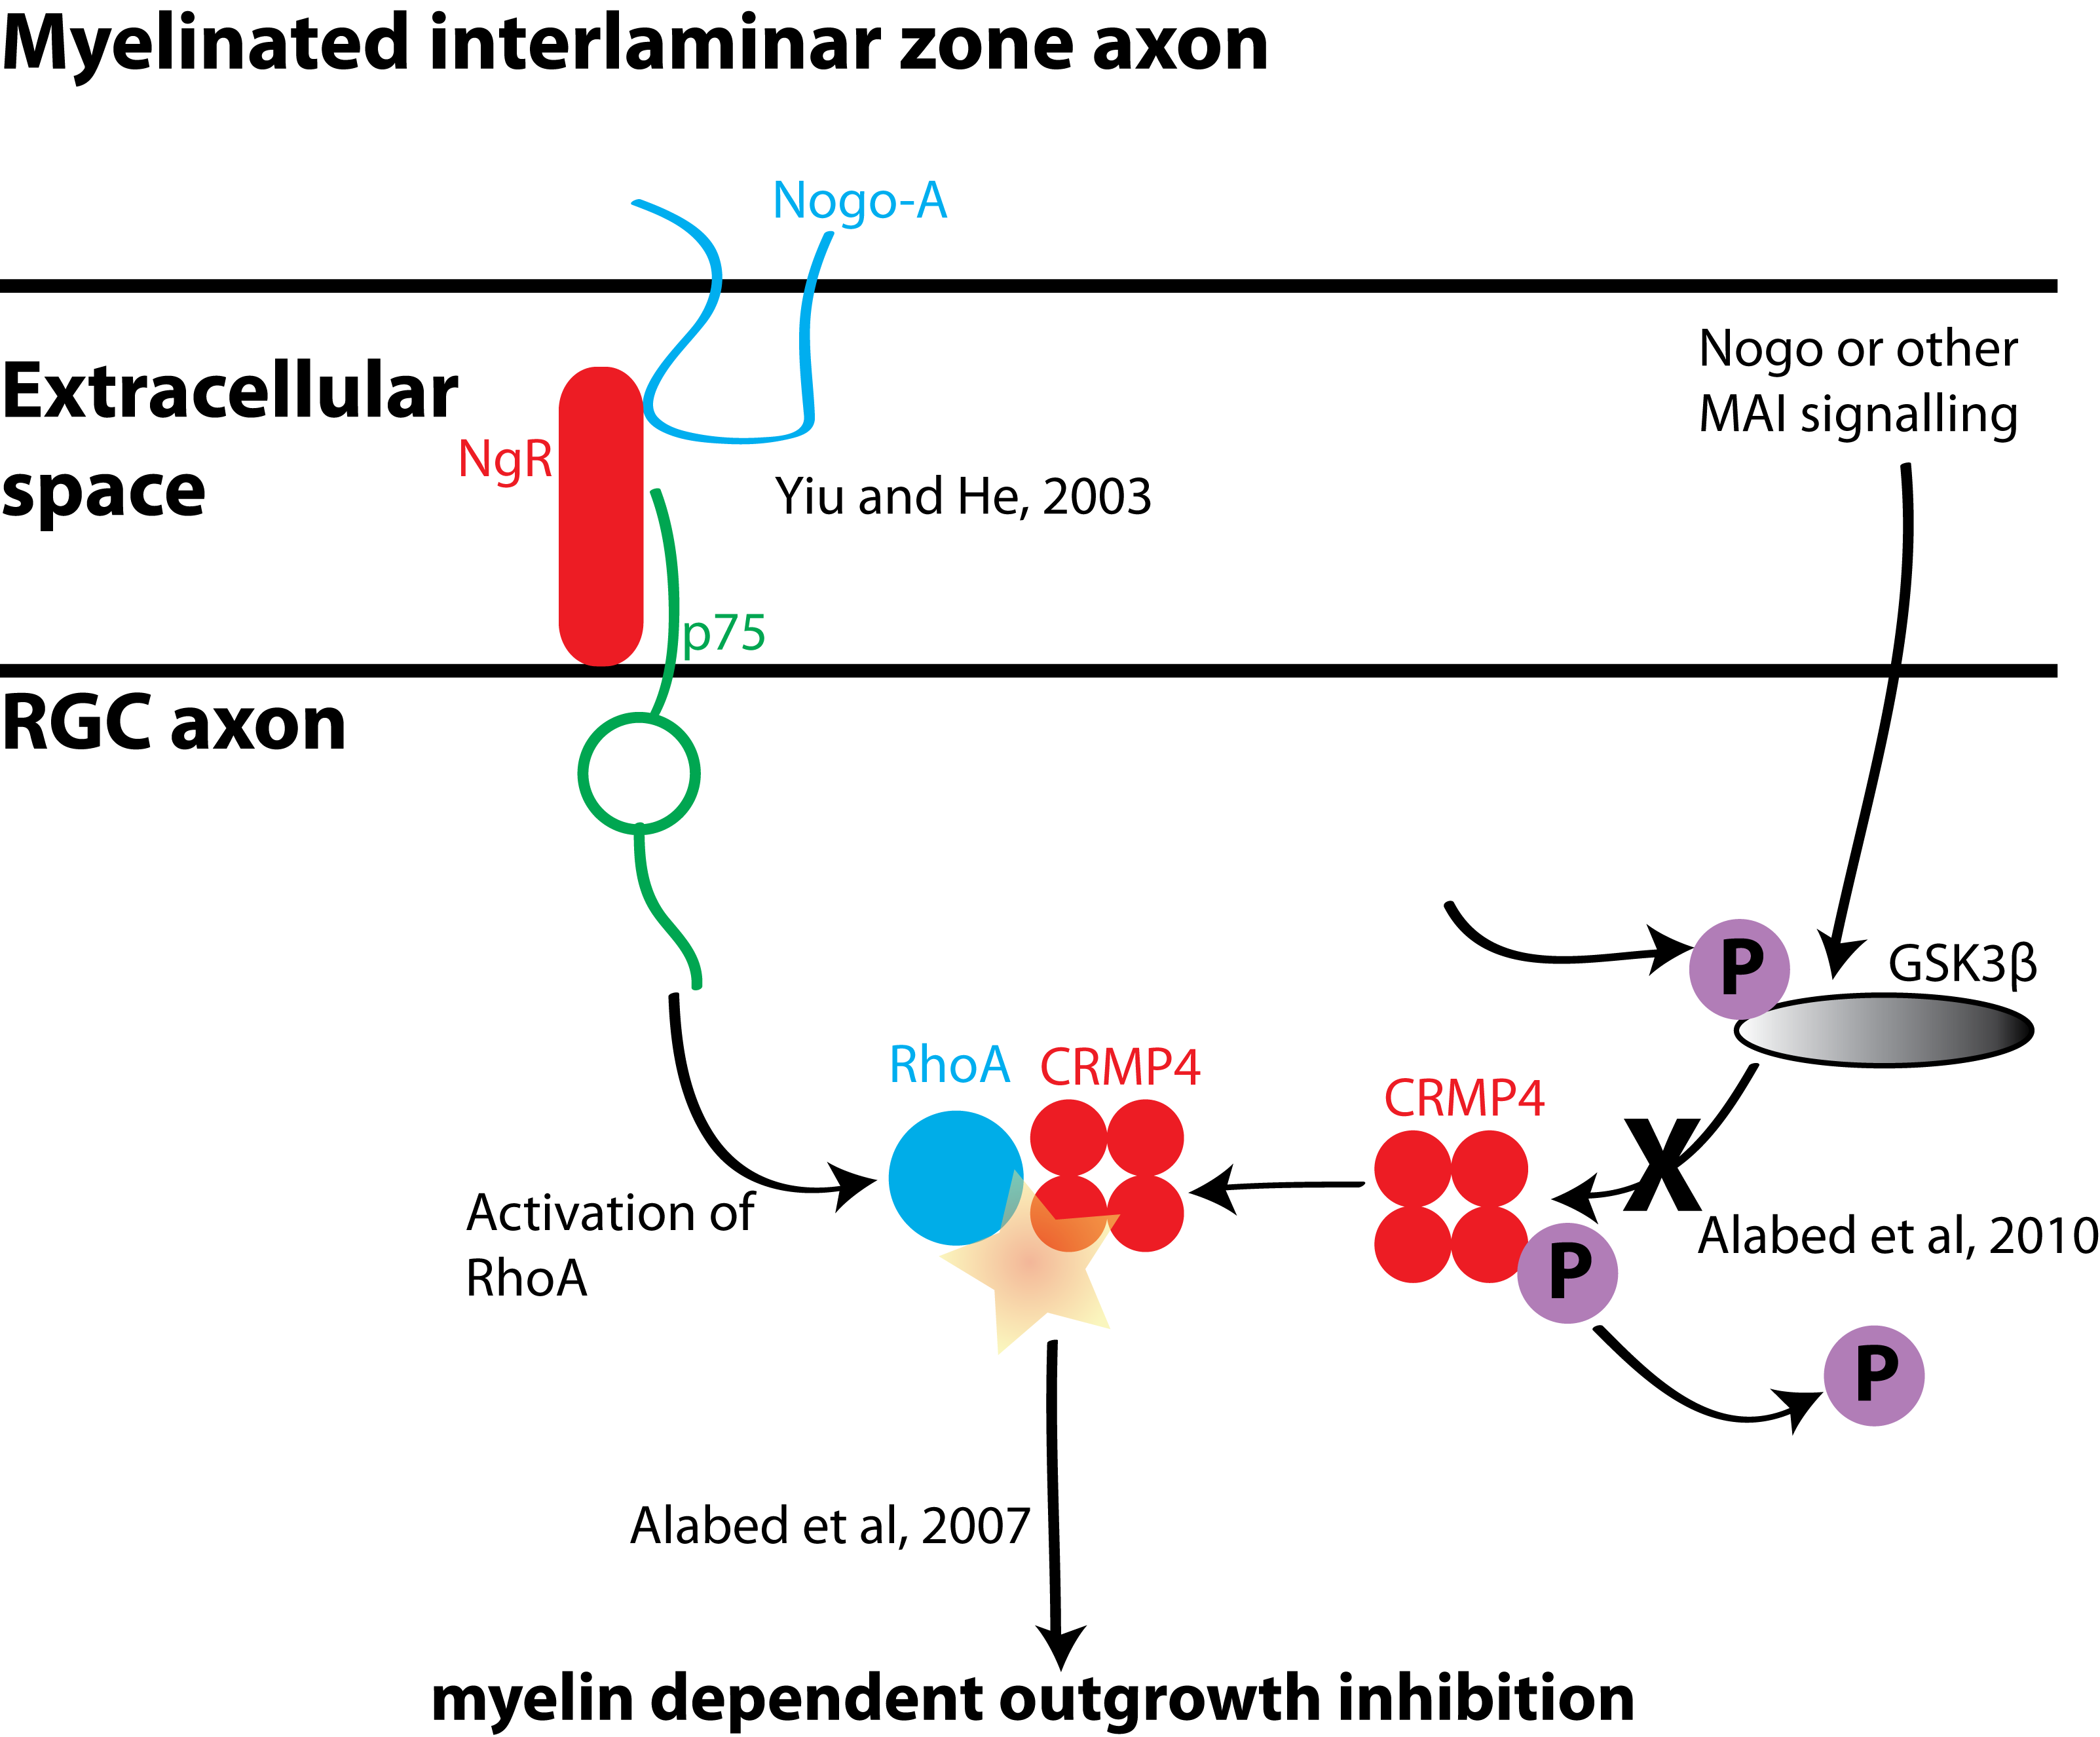
\includegraphics[width=1.0\textwidth]{FigureImages/MAISignals.png}
\end{center}
\caption[MAI signaling through CRMP4 and RhoA results in myelin dependent outgrowth inhibition.]{MAI signaling through CRMP4 and RhoA results in myelin dependent outgrowth inhibition. Nogo-A signaling through the complex of the Nogo receptor (NgR) and p75 results in the activation of RhoA (Yiu and He, 2003).  This activation allows RhoA to bind to CRMP4 (Alabed et al, 2007).  Signaling through Nogo or other myelin associated inhibitors (MAIs) results in the phosphorylation of glycogen synthase kinase 3$\beta$ (GSK3$\beta$).  Phosphorylation inactivates GSK3$\beta$ and leads to a loss of phosphorylation of CRMP4 (Alabed et al, 2010).  Unphosphorylated CRMP4 becomes active and is free to bind with RhoA.  Binding of RhoA and CRMP4 leads to myelin dependent outgrowth inhibition (Alabed et al, 2007).  In the context of the ferret interlaminar zone, MAIs are present on myelinated axons passing through the interlaminar zones and RGC axons expressing CRMP4 could exhibit myelin dependent outgrowth inhibition at interlaminar boundaries through these signaling cascades.}
\end{figure}

\begin{figure}[htb!]
\begin{center}
\leavevmode
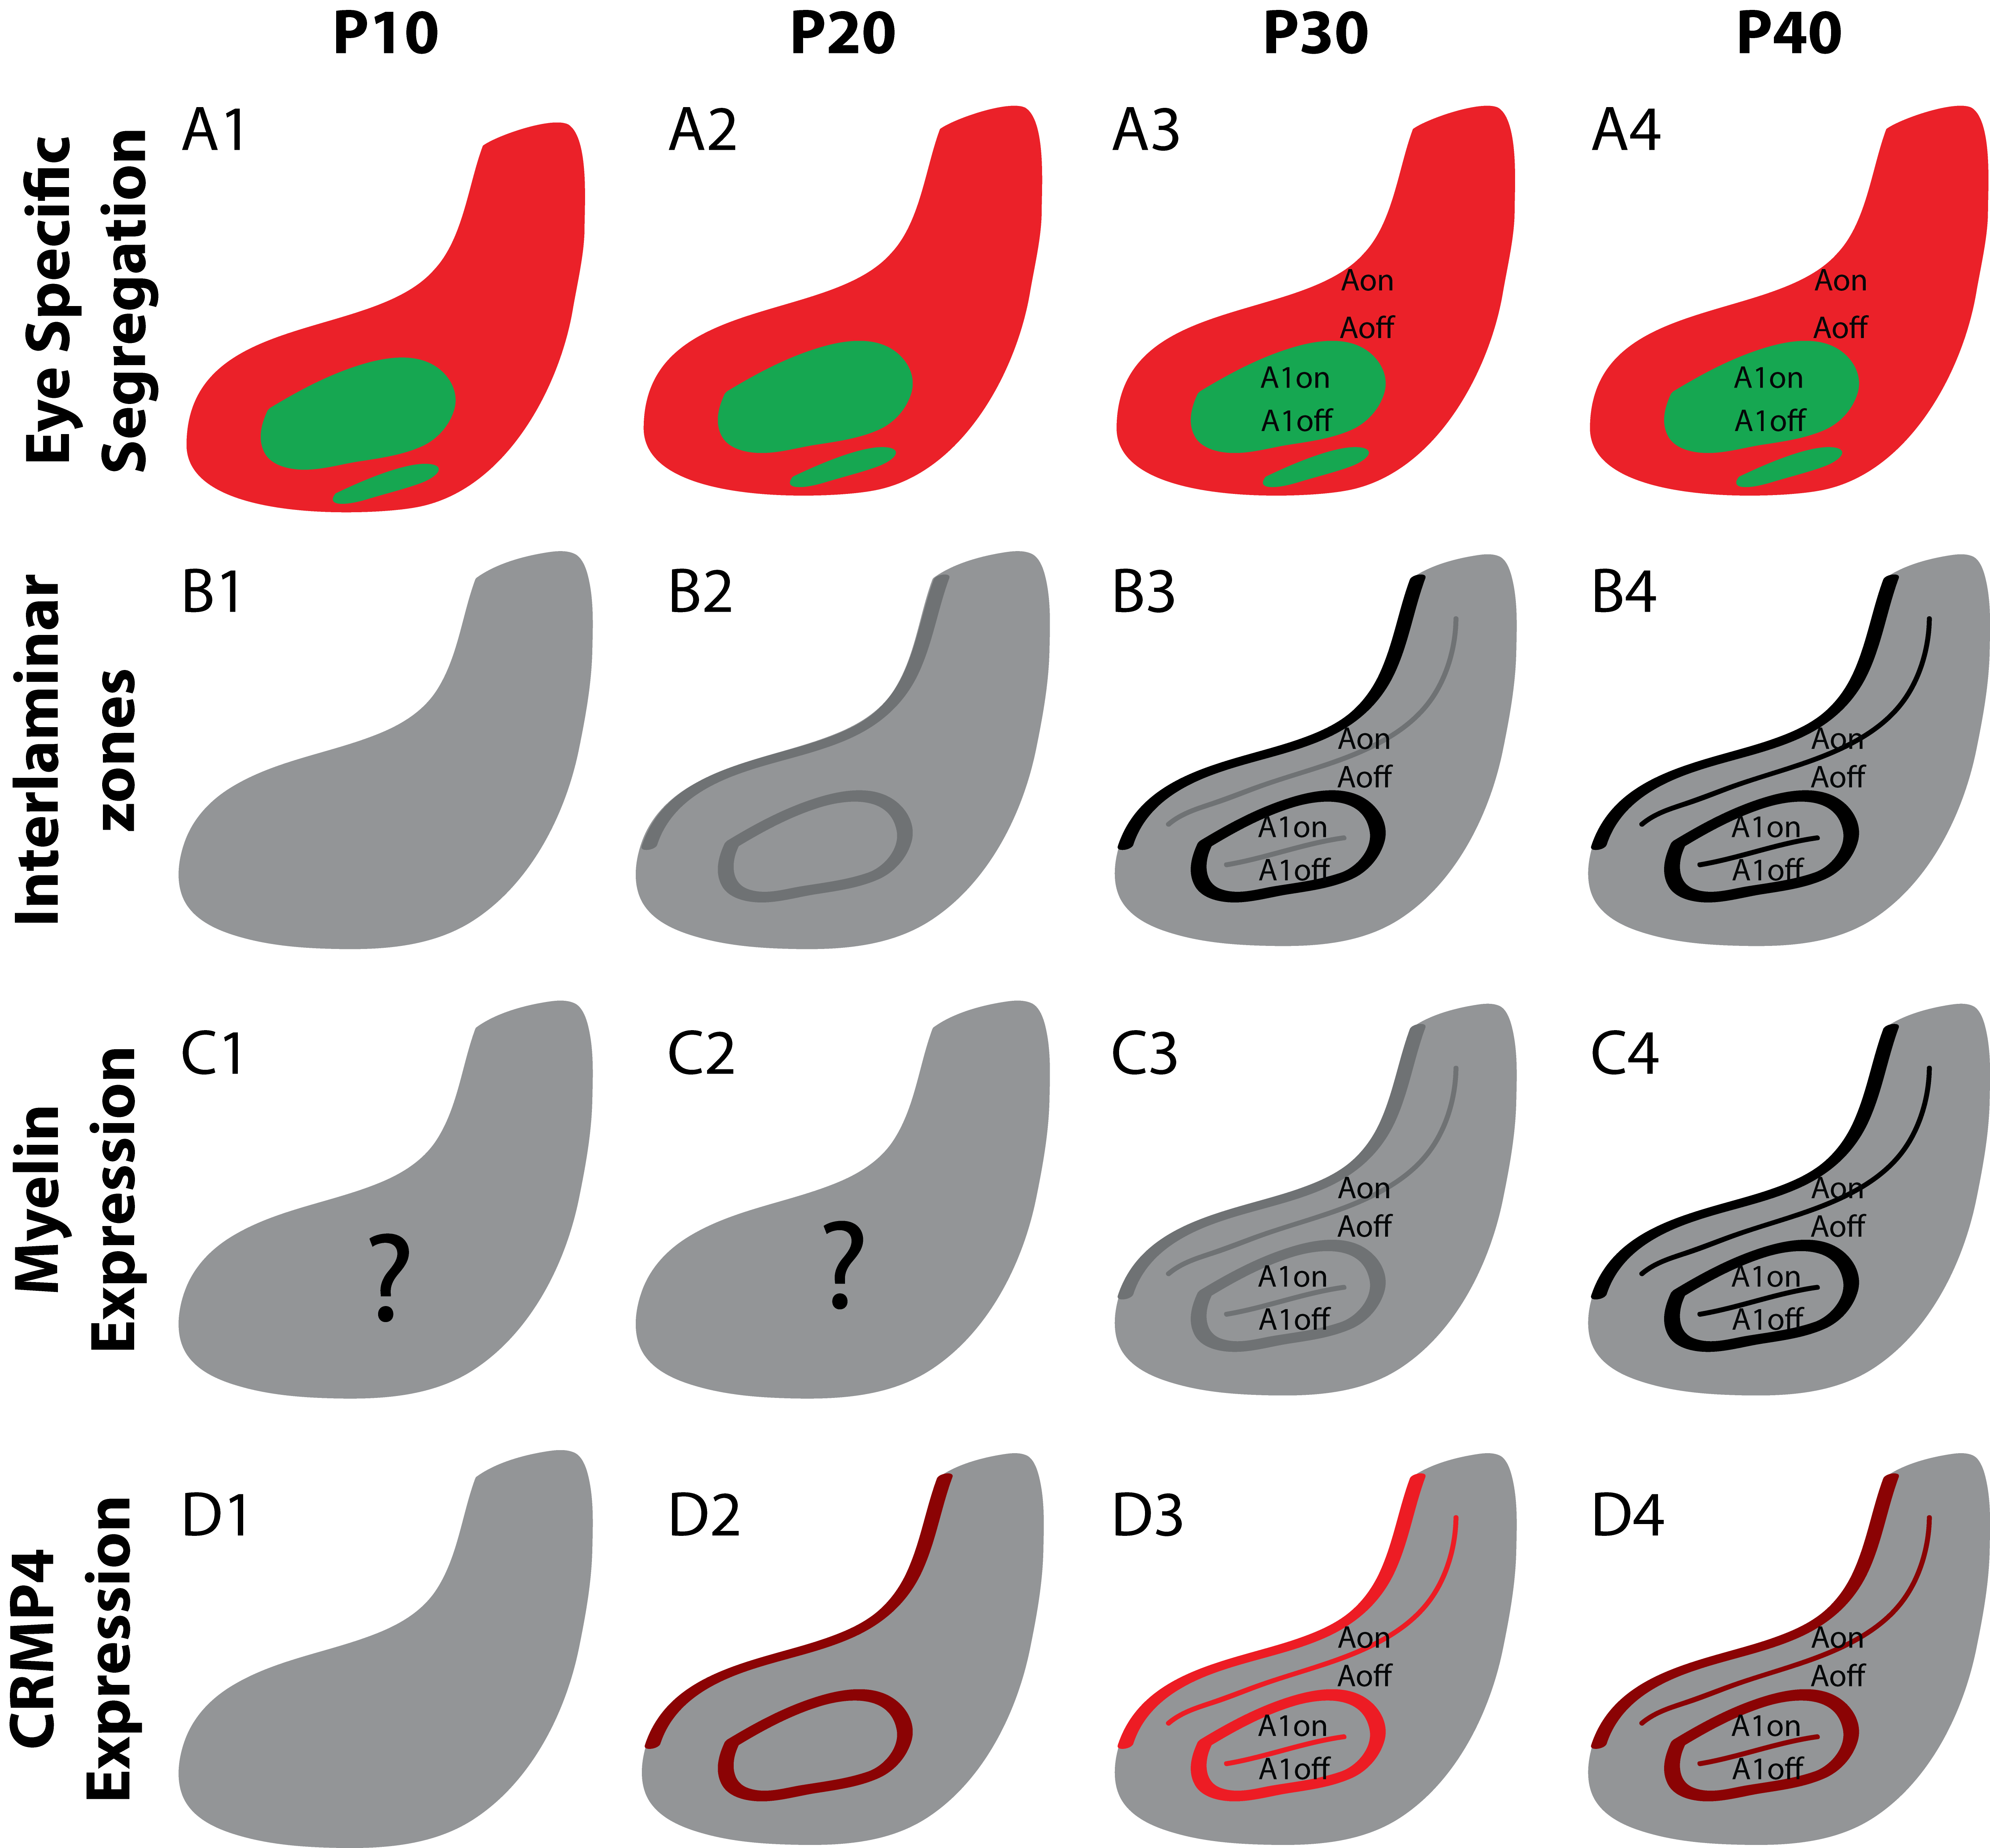
\includegraphics[width=1.0\textwidth]{FigureImages/Chapter5Summary.png}
\end{center}
\caption[Development of eye specific segregation, interlaminar zones, myelination, and CRMP4 expression in the normal ferret LGN.]{Development of eye specific segregation, interlaminar zones, myelination, and CRMP4 expression in the normal ferret LGN. Row A, eye specific segregation is complete by P10 and is maintained throughout adult hood.  ON and OFF sub-domains appear in segregated eye specific lamina by P30. Row B, Interlaminar zones are not present at P10 but begin to develop by P20.  Nascent interlaminar zones mature and minor cell sparse regions at the ON/OFF sub-laminar boundaries appear by P30.  Row C, It is unclear if any myelination is present in the LGN of animals at P10 and P20.  By P30, the interlaminar zones and ON/OFF sub-laminar boundaries zones become myelinated.  This myelination pattern becomes more dense as the animal ages. Row D, CRMP4 expression is absent at P10 and apparent at the interlaminar zones by P20.  By P30, the interlaminar zones and sub-laminar ON/OFF boundaries robustly express CRMP4.  Around P40, CRMP4 expression begins to fade across the nucleus.}
\end{figure}
\pagebreak

%------------------------------------Chapter 5 figs -----------------------------------------------

\subsection{Hypothesis ii: CRMP4 serves as a response factor downstream of semaphorin signaling and mediates growth cone collapse in the cell sparse interlaminar zones.}
The Semaphorin family of proteins includes both secreted and membrane bound proteins that are implicated in both attractive and repellant axon guidance (Raper, 2000).  Canonically, semaphorin signaling is transduced at the cellular membrane through the action of the plexin family of transmembrane receptors.  Different plexin family members bind to different classes of semaphorins (Nakamura et al., 2000).  For the remainder of this section, I will limit my discussion of the semaphorin family to class 3 semaphorins.  Class 3 semaphorins are secreted proteins that bind to a receptor complex composed of plexinA and either neuropilin-1 or neuropilin-2.  PlexinA and one of the two neuropilins are obligate co-receptors for functional class 3 semaphorin signaling (Kolodkin et al., 1997).   Specifically,a class 3 semaphorin, Sema3a, is known to cause growth cone collapse through the intracellular action of CRMP4 (Goshima et al., 1995; Schmidt and Strittmatter, 2007) and as such will be the focus of discussion here. 

To mediate axon dynamics only in the interlaminar zones of the LGN, a diffusible molecule such as Sema3a would have to originate from point sources in the interlaminar zones and not diffuse out of the interlaminar zones into the main layers of the LGN.  It is unlikely that this is the case in the developing LGN for two reasons.  First, the interlaminar zones are very thin.  The width of the interlaminar zone in adult LGNs is no wider than 50�m.  This estimate is conservative and the width of the interlaminar zones is certainly smaller as the LGN is developing and slowly progressing toward the morphology seen in the adult.  It is unlikely that the diffusion of Sema3a would be limited to the interlaminar zones given that a Sema3a molecule originating in a point source in the middle of an interlaminar zone would only need to diffuse 25$\mu$m to encroach upon the main layers of the LGN.  As a a point of reference, molecules close to the size of Sema3a (125 kDa) diffuse through water with a diffusion coefficient of 0.45x10-3 �m2/s (Nauman et al., 2007).  If this diffusion coefficient is assumed for Sema3a in the interlaminar zones of the LGN, it would take 15 hours for a point source of Sema3a at the center of an interlaminar zone to drive Sema3a signaling outside of the interlaminar zone.  The actual diffusion coefficient observed for Sema3a in the interlaminar zones would depend on the influence of the extra cellular matrix in the interlaminar zones.  If Sema3a fails to diffuse as indicated above due to an excess of binding partners or if Sema3a leaves the secreting cell but remains bound to its surface, the diffusion of Sema3a in the interlaminar zones may be much lower than expected. 

Even if it is taken as a given that a point source of Sema3a in the interlaminar zones of the LGN will not result in Sema3a signaling outside of the interlaminar zones, the hypothesis that CRMP4 expression in the interlaminar zones serves to mediate Sema3a signaling suffers from a lack of spatially confined Sema3a sources in the LGN.  Within the LGN, there are different classes of cells that are molecularly distinct from one another.  In the primate, these cells are divided into two major classes, magnocellular and parvocellular.  Different layers in the primate LGN are composed of either magnocelluar or parvocellular cells.  A third, molecularly distinct, set of cells found in the interlaminar zones has also been identified (Livingstone and Hubel, 1984; Hendry and Yoshioka, 1994; Hendry and Reid, 2000).  These cells form the koniocellular pathway in the LGN.  In the cat, the observed cell types of the LGN are X and Y cells.  These cells are physiologically and morphologically distinct from one another.  Unlike the primate,  cell types in the cat LGN are not neatly organized into different laminae (LeVay and Ferster, 1977).  Additionally, the cells in the interlaminar zones of the cat do not appear to have a distinct molecular phenotype.  The ferret LGN resembles the LGN of the cat more than the primate in both its constituent cell types and in its anatomy. As an example, I attempted to identify ferret LGN cells analogous to those reported in the primate koniocellular pathway in a pilot study.  Staining for calcium/calmodulin-dependent protein kinase 2 (CamK2) in the primate LGN reveals cells in the koniocellular pathway.  Staining for CamK2 in the ferret LGN revealed CamK2 positive cells throughout the volume of the LGN.  With the observed homogeneity in cell type across the LGN, it is unlikely that only cells found in the interlaminar zones of the ferret LGN would secrete Sema3a.  It is much more likely that Sema3a secretion would be evenly distributed throughout the nucleus.  

Due to both the spatial precision over which CRMP4 expression occurs in the developing LGN and the lack of a molecularly distinct cell type in the interlaminar zones of the ferret LGN, it is unlikely that CRMP4 serves as a response factor downstream of semaphorin signaling and mediates growth cone collapse in the cell sparse interlaminar zones.

\subsection{Hypothesis iii: CRMP4 serves to modulate calcium signaling in RGC axon terminals in the cell sparse interlaminar zones}
Recent studies have shown that CRMP2 has an alternative role in synaptic plasticity beyond its typical role in growth cone dynamics.  CRMP2 has been shown to interact with the N-type presynaptic Ca2+ channel (CaV2.2) and this interaction serves to modulate the of Ca2+ current moving through presynaptic CaV2.2 channels (Brittain et al., 2009).  Modulation of calcium channels influences the action of presynaptic calcium flux in turn modulates neurotransmitter release at the synapse (Catterall and Few, 2008).  Specifically, an increase in CRMP2 levels leads to an increase in calcium flux and a consequent increase in neurotransmitter release. It is unknown if the observed interaction with CaV2.2 and CRMP2 is specific to CRMP2 or if it may be a general property of the CRMP family.  If CRMP4 is also capable of modulating synaptic plasticity, CRMP4 may serve to modulate calcium signaling in RGC axon terminals in the cell sparse interlaminar zones and thus modulate synaptic plasticity in the cell sparse interlaminar zones through an increase in neurotransmitter release.  An increase in neurotransmitter release could lead to increase synaptic efficacy in portions of the LGN with high local calcium concentrations through the action of CRMP4.  For this hypothesis to hold there should be a difference in calcium signaling between the cell sparse interlaminar zones and the main laminae of the LGN.  This difference would then provide a substrate upon which CRMP4 could serve to shape the projections of RGC into the LGN.  Under this scheme CRMP4 expression at the interlaminar zones would result in increased sensitivity to different local calcium levels and thus larger differences in the synaptic strength of developing synapses in the interlaminar zones and main LGN layers.  If local calcium levels were lower in the interlaminar zones than the main LGN layers, this scheme could lead to a strengthening of synapses onto the main LGN laminae a weakening of synapses onto the interlaminar zones.  Differential synaptic plasticity of this kind could assist in fine tuning laminar boundaries in the LGN. 

In order to test this hypothesis, it will be necessary to characterized the magnitude of calcium flux across the LGN.  Characterization of the LGN in this way could be carried out using calcium imaging in LGN slice preparations.  If the interlaminar zones of the LGN are identified either directly by characterization of cytoarchitecture or indirectly by fluorescent tracer injections into the retina, an imaging location could be chosen such that it includes an interlaminar zone as well as the bordering main LGN laminae.  Calcium flux in response to stimulation across the slice could then be visualized in order to determine if the interlaminar zones behave differently from the main LGN laminae. 

I do not favor this hypothesis due to the fact that CRMP4 has not definitively been shown to interact with calcium channels at the synapse or hold sway over any other synaptic properties directly.   The CRMP family is defined by a common structural similarity and is actually composed of members that have a significant variation around a the base CRMP structure.  As a result, the family has been shown to participate in a wide variety of functions (Schmidt and Strittmatter, 2007).  Not all members of the CRMP family share all of the functions of the family and it is not a good assumption that an atypical CRMP function such as interaction with CaV2.2 channels is common to all CRMPs.  Without direct evidence for an interaction of CRMP4 with calcium signaling or other synaptic phenomenon, I do not find it likely that CRMP4 serves to modulate synaptic plasticity directly in the interlaminar zones.

\section{Conclusions}
\subsection{Specific conclusions}
In this dissertation, I have outlined a strategy for the characterization of molecular correlates of visual development.  Specifically, I present a novel strategy for the exploration of the molecular basis of ocular dominance.  The study of visual development in this way led to the characterization of a novel marker for LGN development, CRMP4.  I show that CRMP4 expression is both developmentally regulated and subject to manipulation through classic alterations of LGN anatomy through enucleation and activity modulation in the retina.  CRMP4 expression covaries with the expression of myelin in the LGN and CRMP4 may serve to fine tune the laminar wiring of the LGN through myelin dependent outgrowth inhibition.  Alternative explanations of the mechanism of CRMP4 action in the developing LGN include mediation of semaphorin signaling or the mediation of synaptic plasticity through an interaction with calcium signaling.  Definitive proof of the mechanism of CRMP4 action in the developing LGN will require additional experimentation beyond the scope of this dissertation. 

It is also worth noting that the methods presented here for the molecular characterization of the visual system are applicable to other modular neural systems.  In many neural systems, it is possible to generate pairs of samples that represent closely related functional modules.  These pairs of modules could easily be assayed using the methods presented here.  As an example, many of the primary sensory modalities could be examined using similar approaches to what is seen here.  It would be straight forward extension of the methods presented here to characterize the molecular compliments of different barrels in S1 of the rodent, different tonotopic representations in auditory cortex, or different odor representations in the olfactory bulb, to list a few.  In all of these cases, an adaptation of the tissue sampling paradigms presented in this dissertation followed by a differential screen using 2D-DIGE or other screening system could lead to a novel perspective on the influence of molecular cues in these systems.

\subsection{General conclusions}
Historically, much of neural development was viewed as a result of endogenous and externally driven activity paradigms.  In this view the remarkable reliability of neural anatomy across both individuals and generations was thought to be a result of stereotyped environmental influences on the nervous system.  From the view of a single neuron, the pattern of activity that it receives and the pattern of activity that its potential synaptic partners display were thought to be the driving forces behind wiring decisions.  This perspective has been at the root of many successes and breakthroughs in our understanding of neural function.  However, the story of neural development is much more complex than it would seem when viewed simply as a result of neural activity.  Molecular influences on neural systems have come to be known as driving forces in development as well.  From the perspective of a single neuron, the full complement of its molecules and that of its potential synaptic partners augments wiring decisions in the face of activity paradigms.  These two developmental schemes appear to be at odds with one another, but I believe that they are in fact synergetic. 

Over the last two decades, there has been an massive proliferation of methods aimed at genetic and molecular characterization of biological systems and the field of developmental neuroscience has borrowed heavily from these tools.  In the most general sense, the work presented in this dissertation represents an additional borrowing.  It is my belief that application of tools such as those presented in this dissertation to the study of neural development will paint a much more holistic picture of neural development than what is found in many current textbooks.  Rather than viewing neural development through the lens of activity dependent mechanisms or molecular mechanisms, we will come to realize that the actual mechanics of neural development are a marriage of both.  Activity and molecular influences on neural systems will lose their discrete labels as we study the two systems in tandem.  We will see that one influences the other and feeds back onto itself.  There is a sort of beautiful completeness to this perspective on the operation of neural systems.